\chapter{Novel Work} \label{novelw}

In this section the work completed so far will be presented. Two main areas of the systematic review process has been focused on: stopping criteria and indexing/querying PubMed.



\subsection{CLEF 2017 Runs} \label{clefRuns}

For the CLEF 2017 Technologically Assisted Reviews in Empirical Medicine \cite{Kanoulas12017}, participants were expected to submit runs for ranking documents. Participants were given complex boolean queries that could be used for extracting relevant information to rank the documents. These runs were later released for public access \footnote{https://github.com/CLEF-TAR/tar/tree/master/2017-TAR/participant-runs}

\begin{table}[!htbp]
\scalebox{0.75}{
\centering
\caption{The 6 runs sampled from the CLEF 2017 task.}
\label{my-label}
\begin{tabular}{|l|l|l|}
\hline
Run                  & Description                                                                    & Reference                                     \\ \hline
Sheffield-run-2      & Sheffield-2 used tfidf similarity along with standard pre-processing           & \cite{Alharbi2017}           \\ \hline
Waterloo A-rank-cost & Waterloo used a baseline model implementation from the TREC Total Recall Track & \cite{cormack2017technology} \\ \hline
Waterloo B-rank-cost & -                                                                              & \cite{cormack2017technology} \\ \hline
auth run-1           & AUTH used a learning-to-rank approach and used both batch and active learning  & \cite{Anagnostou2017clef}    \\ \hline
auth run 2           & -                                                                              & \cite{Anagnostou2017clef}    \\ \hline
ntu run-1            & Used convolutional neural networks (CNN)                                       & \cite{lee2017clef}           \\ \hline
ucl full-text        & Used a deep learning model architecture                                        & \cite{singh2017identifying}  \\ \hline
\end{tabular}
}
\end{table}


We have taken 6 ranking sets of which are of different quality. The Waterloo and AUTH ranks are the best rankings followed by Sheffield. The UCL and NTU submissions feature poorer quality rankings.

CLEF 2017 runs will follow a format similar to the example below. The most important information being the topic id and the document id.


\begin{tcolorbox} \label{scoreExample}
CD010775 NF 19307324 1 0.27152011529138564 Test-Data-Sheffield-run-2 
\end{tcolorbox}

Results can be evaluate using qrel files, supplied as part of the CLEF 2017 data. These files contain relevant documents for each topic, and are formatted as follows:

\begin{tcolorbox}
CD008803     0  21467181     0  \\
CD008803     0  20872357     1  \\
CD008803     0  23837966     0 
\end{tcolorbox}

Where the 1 or 0 on the right side indicates if the document is relevant for a study.



\section{Baseline Approaches to Stopping} \label{baselineapp}

We can now establish some baseline approaches for finding stopping points. Approaches are heavily dependant on the initial rankings of the document collection, and naturally assume more relevant documents feature towards the start of the collection.

\subsection{Oracle Scores} \label{oracleScores}

Looking at the oracle scores for each set of rankings will tell us the best we can possibly for do this task.  We will assume we are satisfied with 70\% recall. These scores are calculated as the minimum amount of effort that could be made to achieve 70\% recall. Results are taken as averages over all topics.

\begin{table}[H]

\centering
\begin{tabular}{|c|c|c|c|c|} 
\hline
 Submission & recall & reliability & effort  \\ 
 Test\_Data\_Sheffield-run-2 & 0.7 &	1.0	&	0.11 \\ 
 Waterloo A-rank-cost & 0.7 &	1.0	&	0.07 \\ 
 Waterloo B-rank-cost & 0.7 &	1.0	&	0.06 \\ 
 auth run-1 & 0.7 &	1.0	&	0.08 \\ 
 auth run-2 & 0.7 &	1.0	&	0.09 \\ 
 ntu run-1 & 0.7 &	1.0	&	0.4 \\ 
 ucl full-text & 0.7 &	1.0	&	0.67 \\ 
 \hline
\end{tabular}

\caption{Lowest effort possible to find 70\% of relevant documents. }

\end{table}

These scores highlight the importance of the ranking methods for finding a stopping point. The best performer, Waterloo B-rank-cost needs just 6\% effort to hit 100\% reliability. The worst performer, ucl full-text requires 67\% effort for the same level of reliability.


\subsection{Percentage cut-off method} \label{perCutOffMethod}

As a first approach we could simply take a cut of the document collection and evaluate how many relevant documents we have retrieved. This likely to be very dependant on the initial rankings of the document collection. 

\begin{table}[!htbp]
\scalebox{0.75}{
\centering
\caption{Comparison of results between rankings when looking at a percentage of the ranked documents.}
\label{my-label}
\begin{tabular}{|l|l|l|l|l|l|l|l|l|l|l|l|l|l|l|l|}
\hline
\% of Documents      & \multicolumn{3}{l|}{10\%}     & \multicolumn{3}{l|}{25\%} & \multicolumn{3}{l|}{50\%} & \multicolumn{3}{l|}{75\%} & \multicolumn{3}{l|}{90\%} \\ \hline
Run                  & Recall & Reliability & Effort & -       & -      & -      & -       & -      & -      & -       & -      & -      & -       & -      & -      \\ \hline
Sheffield-run-2      & 0.49   & 0.16        & 0.10   & 0.74    & 0.66   & 0.25   & 0.91    & 0.93   & 0.50   & 0.98    & 1.00   & 0.75   & 0.99    & 1.00   & 0.90   \\ \hline
Waterloo A-rank-cost & 0.80   & 0.6         & 0.10   & 0.91    & 0.93   & 0.25   & 0.98    & 1.00   & 0.50   & 0.99    & 1.00   & 0.75   & 0.99    & 1.00   & 0.90   \\ \hline
Waterloo B-rank-cost & 0.73   & 0.63        & 0.10   & 0.90    & 0.93   & 0.25   & 0.98    & 1.00   & 0.50   & 0.99    & 1.00   & 0.75   & 0.99    & 1.00   & 0.90   \\ \hline
auth run-1           & 0.72   & 0.63        & 0.10   & 0.90    & 0.93   & 0.25   & 0.97    & 1.00   & 0.50   & 0.99    & 1.00   & 0.75   & 0.99    & 1.00   & 0.90   \\ \hline
auth run 2           & 0.68   & 0.60        & 0.10   & 0.88    & 0.9    & 0.25   & 0.97    & 1.00   & 0.50   & 0.99    & 1.00   & 0.75   & 0.99    & 1.00   & 0.90   \\ \hline
ntu run-1            & 0.19   & 0.00        & 0.10   & 0.39    & 0.06   & 0.25   & 0.62    & 0.43   & 0.50   & 0.83    & 0.83   & 0.75   & 0.91    & 0.93   & 0.90   \\ \hline
ucl full-text        & 0.08   & 0.00        & 0.10   & 0.22    & 0.00   & 0.25   & 0.46    & 0.03   & 0.50   & 0.70    & 0.70   & 0.75   & 0.87    & 0.93   & 0.90   \\ \hline
\end{tabular}
}
\end{table}

All scores are averaged over the entire ranking set.

Sheffield has an average recall of 0.49 by the time 10\% of the documents have been observed. Waterloo has achieved 80\% recall by this point. After looking through 25\% of the rankings Waterloo and AUTH have achieved around 90\% recall of documents.

The limitation of this approach is the effort required looking through documents is still high. We want to lower this effort as much as possible, whilst only having to observe relevant documents.


\subsection{Similarity score cut-off method} \label{simScoreMethod}

A similarity score method will assume each document in the rankings has a score associated with it. Consider the ranking format described in \ref{clefRuns}. The 5th column describes a similarity between the document and the query. Similarity scores gradually decline as we descend down the rankings. For this experiment we only use the Sheffield rankings.

The similarity score can be used derive a stopping point. This method works by looking at documents $D_i$ and $D_{i+1}$ and determining if the difference between the similarity scores has become too large. This method will work on the basis that documents that are no longer relevant will have a sudden drop in score such that we can identify this as our stopping point.

\begin{equation}
	  Difference(D_i, D_{i+1}) > C
\end{equation}

Where difference returns a score of how close document $D_i$ and $D_{i+1}$ are together and $C$ is a cut-off constant. We can expand this to an example:

\begin{equation}
	  (1 -(0.73 / 0.75)) * 100 > 0.015
\end{equation}

Here we are saying if the two documents' scores are above 1.5\% then we should stop looking down the rankings.


\begin{table}[H]
\centering
\begin{tabular}{|c|c|c|c|c|} 
\hline
 $dif(D_i, D_{i+1})$ & recall & reliability & effort  \\ 
 0.01\% & 0.025 &	0.000	&	0.0023 \\ 
 0.05\% & 0.120 &	0.100	&	0.100 \\ 
 1\% & 0.359 &	0.333	&	0.333 \\ 
 2\% & 0.880 &	0.860	&	0.860 \\ 
 5\% & 1.000 &	1.000	&	1.0000 \\ 
 \hline
\end{tabular}

\caption{Similarity cut-off comparison for stopping for Test\_Data\_Sheffield-run-2. Using cosine similarity scores.}
\end{table}

These results are highly sensitive to the similarity score and show it's difficult to use this score as an affective measure for stopping. We found similarity scores rarely have sudden drops in values, making it difficult to use this method to identify a stopping point.

As an alternative approach, we can look at just the top document $D_1$, and compare it to the succeeding documents $D_{1+i}$ in the rankings. We can formulate this as follows:

\begin{equation}
	  Difference(D_1, D_{1 + i}) > C
\end{equation}

\begin{table}[H]
\centering
\begin{tabular}{|c|c|c|c|c|} 
\hline
 $dif(D_1, D_{1+i})$ & recall & reliability & effort  \\ 
 10\% & 0.048 &	0.000	&	0.004 \\ 
 20\% & 0.063 &	0.000	&	0.007 \\ 
 30\% & 0.113 &	0.000	&	0.152 \\ 
 40\% & 0.191 &	0.030	&	0.029 \\ 
 50\% & 0.319 &	0.060	&	0.063 \\
 60\% & 0.460 &	0.200	&	0.113 \\ 
 70\% & 0.638 &	0.433	&	0.210 \\ 
 80\% & 0.841 &	0.800	&	0.387 \\ 
 90\% & 0.979 &	1.000	&	0.679 \\ 
 100\% &1.000 &	1.000	&	1.000 \\  
 \textbf{85.5\%} & \textbf{0.934} &	\textbf{1.000}	&	\textbf{0.538} \\  
 \hline
\end{tabular}

\caption{Similarity cut-off comparison for stopping for Test\_Data\_Sheffield-run-2. Using cosine similarity scores. Compares first document to succeeding documents}
\end{table}

We found results to be much better when using the first document to look for a stopping point. 85.5\% difference in first and subsequent documents was found to be the point for hitting 1.0 reliability. This comes at the expense of making just over 50\% effort.

\section{Sample Method to Stopping} \label{samplemethods}

The limitations of the methods presented in \ref{baselineapp} is that they they still require looking through a large volume of documents.

The approaches in this section will use sampling methods. These approaches assumes we have sensible ranking algorithm for returning documents for a query. They work by generating a sample set, which acts as our model for predicting a stopping point.

The first step is to generate a sample set. We used an interval method for generating our set, i.e select every $N$th document. The intuition being that the distribution of relevant document in the sample set, should be similar to that of the real set of relevant documents. This makes it suitable to use as a model. 


\iffalse
A limitation of this sampling method is that for topics with very few documents it is easy for a sample to miss many of them. This creates a subset set bias, where one set contains a larger percentage of relevant documents. Consider a query that returns 10000 candidate documents of which only 10 have been pre-determined to be relevant. Its not too unlikely that a randomly sampled subset would contain 0 relevant documents. We can use the following equation to tell us how much information we can take from a pre-evaluated topic:

\begin{equation}
I = \frac{rel(T_i)}{|T_i|}
\end{equation}

Where $T_i$ is a given topic and $rel$ computes the number of relevant documents for that topic. Therefore $I$ is telling us how useful the topic is at fitting a curve. We can take the average simply by taking the mean of $I$ across all topics:

\begin{equation}
Usefullness = \frac{\sum{I}}{|T|}
\end{equation}
\fi


\subsection{Curve Fitting}

Our first approach is to fit a non-linear curve against a sample set. We used a sample size of 3.

\begin{equation}
F(x) = n - a\exp^{-kx}
\end{equation}

Where $a$, $k$ and $n$ are learnt weights and $x$ is an associated return rate for a document. We generate the curve using the non-linear least squares algorithm \cite{leastsqures}. 


\iffalse
We can visualise the curve along with the confidence intervals. The Y axis is the predicted number of relevant documents for the topic. X axis shows the true number of documents returned for the query. 

\begin{figure}[H]
\center
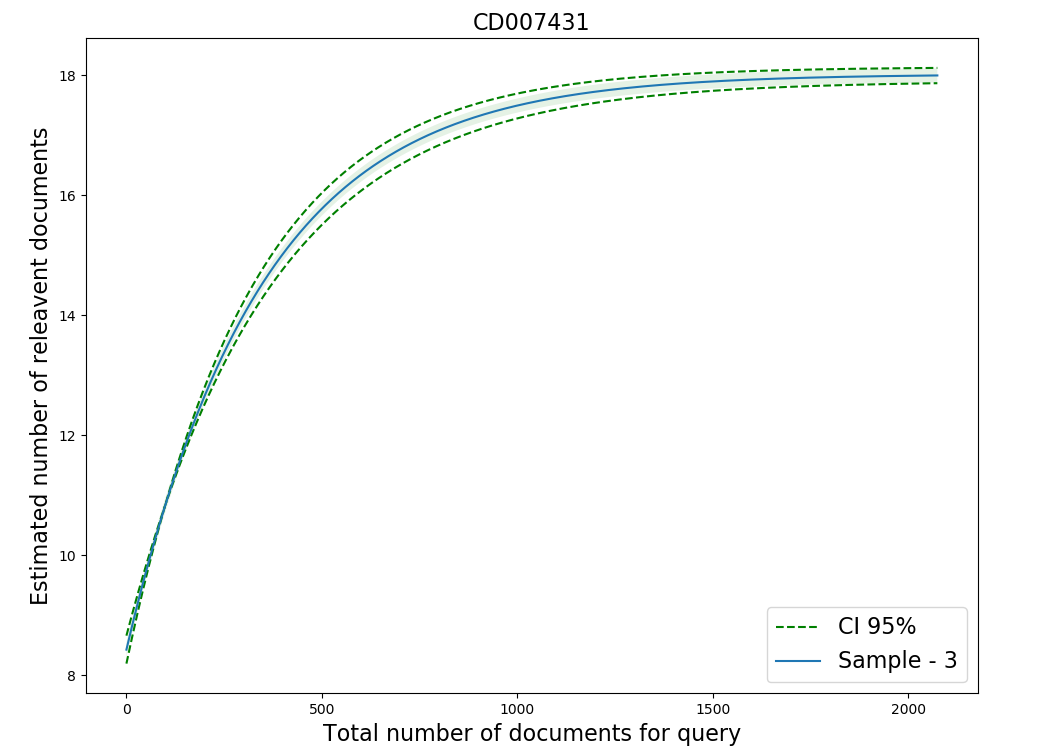
\includegraphics[width=10cm]{figures/curve_fit_example.png}
\caption{Example of fitting a curve for a topic using sampling}
\end{figure}

\begin{table}[H]
\centering
\begin{tabular}{|c|c|c|c|} 

 \hline
 sample size & recall & reliability & effort  \\ 
 1 & 0.91 &	0.96	&	1 \\ 
 3 & 0.66 & 0.5	&	0.48 \\ 
 5 & 0.481 & 0.33	&	0.315 \\ 
 \hline
\end{tabular}
\caption{Comparison of different sample intervals against recall and effort. Ranking Method: Test\_Data\_Sheffield-run-2 \cite{Alharbi2017}}

\end{table}

\fi


\subsubsection{Curve Predictions}

\iffalse
\begin{table}[H]
\centering
\begin{tabular}{|c|c|c|c|c|} 

 \hline
 Submission & recall & reliability & effort & topics sampled  \\ 
 Test\_Data\_Sheffield-run-2 & 0.68 &	0.53	&	0.50 & 30 \\ 
 Waterloo A-rank-cost & 0.70 & 0.46	&	0.44 & 30 \\ 
 Waterloo B-rank-cost & 0.70 & 0.46	&	0.40 & 30 \\ 
 auth run-1 & 0.74 & 0.53	&	0.43 & 30 \\ 
 auth run-2 & 0.70 & 0.50	&	0.43 & 30 \\ 
 ntu run-1 & 0.71 & 0.43	&	0.68 & 30 \\ 
 ucl full-text & 0.86 & 0.8	&	0.91 & 30 \\ 
 \hline
\end{tabular}
\caption{Evaluation of curve fitting for different CLEF 2017 runs. Sample size = 3. Results are taken as averages over all topics for search method. No topic cut-off}

\end{table}
\fi


The number of topics was reduced down from 30 to 23 using a cut-off parameter. This reduces some of topics that contain fewer relevant documents and do not generate suitable prediction curves. We used a cut-off parameter of 0.5\%. This can be read as the number of relevant documents in a document collection must be atleast 0.5\%

We also include a confidence interval evaluation for lower bounded range of a $3\sigma$ confidence interval. The key advantages of using a curve as  method of evaluating stopping criteria is being able to make use of this confidence interval in a real systematic review. In the context of a systematic reviewers at the data filtering stage, we could specify that the system is 95\% certain that 70\% of relevant documents have been found. At which point the reviewer can decide if its worth continuing to look at documents.

\begin{figure}[H]
\center
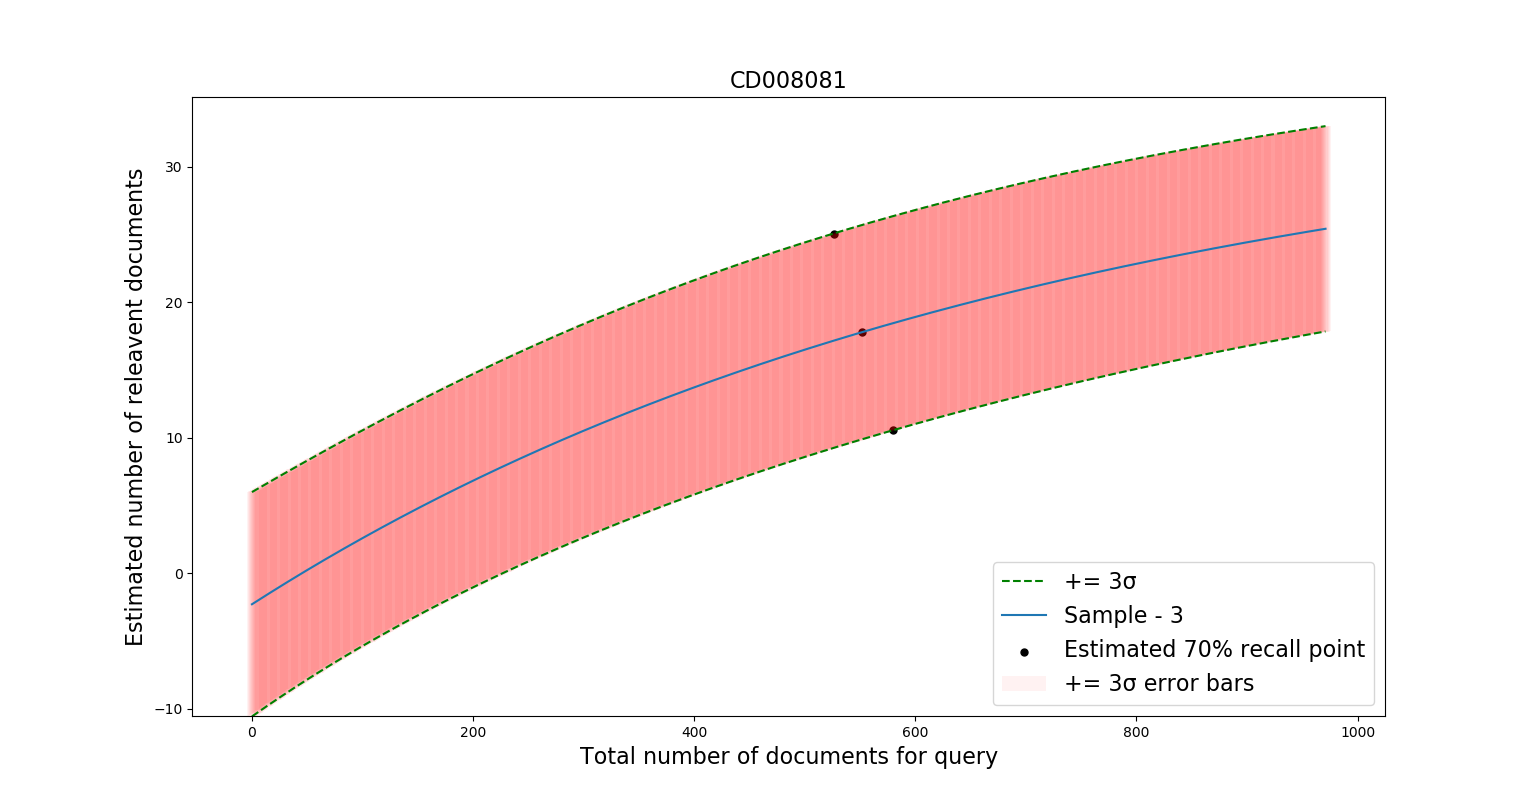
\includegraphics[width=17cm]{figures/cf_example.png}
\caption{Example of a prediction curve for topic CD008081. Confidence bars are included over $3\sigma$. Estimated point of hitting 70\% denoted by black point.}
\end{figure}

\begin{table}[H]
\scalebox{1}{
\centering
\begin{tabular}{|c|c|c|c|c|} 

 \hline
 Submission & recall-lower & reliability-lower & effort-lower & topics sampled  \\ 
 Test\_Data\_Sheffield-run-2 & 0.69 \, 0.74, &	0.52 \, 0.60	&	0.48 \, 0.51 & 23 \\ 
 Waterloo A-rank-cost & 0.71 \, 0.73, &	0.47 \, 0.47	&	0.43 \, 0.44 & 23 \\ 
 Waterloo B-rank-cost & 0.71 \, 0.75, &	0.52\, 0.82	&	0.41\, 0.43 & 23 \\ 
 auth run-1 & 0.72 \, 0.74, &	0.52 \, 0.60	&	0.41 \, 0.42 & 23 \\ 
 auth run-2 & 0.70 \, 0.72, &	0.52 \, 0.60	&	0.42 \, 0.43 & 23 \\ 
 ntu run-1 & 0.76 \, 0.74, &	0.56 \, 0.52	&	0.72 \, 0.70 & 23 \\ 
 ucl full-text & 0.86 \, 0.94, &	0.82 \, 0.86	&	0.91 \, 0.95 & 23 \\ 
 \hline
\end{tabular}
}
\caption{Evaluation of curve fitting for different CLEF 2017 runs. lower = lower-bound confidence interval. Sample size = 3. Results are taken as averages over all topics for search method. with 0.5\% cut-off}

\end{table}

We have deliberately compared two of the better participant rankings (Waterloo and auth) and two of the lower performers (ntu and ucl). We can see the quality of the initial rankings significantly influences the performance of our stopping criteria. This suggests there is a important relationship between using a curve to predict a stopping point and how good the initial ranking of documents is. 

Some of the ranking methods struggle to produce curves and when combined with a cut-of parameter produce become not worth considering in our evaluation. In this situation we simply returned everything for the given topic, resulting in 100\% recall at the expense of 100\% effort.


\subsection{Gaussian Process Fitting}

As an alternate approach to fitting a simple curve, we can apply a Gaussian Process (GP) \cite{ebden2008gaussian}. We will apply a constant kernel plus a squared-exponential kernel. GP was implemented using scikit learn classes. \footnote{http://scikit-learn.org/stable/modules/gaussian\_process.html}


\begin{table}[H]
\scalebox{1.0}{
\centering
\begin{tabular}{|c|c|c|c|c|} 

 \hline
 Submission & recall-lower & reliability-lower & effort-lower & topics sampled  \\ 
 Test\_Data\_Sheffield-run-2 & 0.73 \, 0.73, &	0.73 \, 0.73	&	0.50 \, 0.50 & 23 \\ 
 
 
 Waterloo A-rank-cost & 0.70 \, 0.70, &	0.40 \, 0.40	&	0.42 \, 0.42 & 23 \\ 
 
 
 Waterloo B-rank-cost & 0.73 \, 0.73, &	0.71 \, 0.71	&	0.41 \, 0.41 & 23 \\ 
 
 
 auth run-1 & 0.74 \, 0.75, &	0.56 \, 0.60	&	0.42 \, 0.42 & 23 \\ 
 
 
 auth run-2 & 0.72 \, 0.73, &	0.52 \, 0.52	&	0.42 \, 0.42 & 23 \\ 
 
 
 ntu run-1 & 0.67 \, 0.67, &	0.40 \, 0.40	&	0.64 \, 0.64 & 23 \\ 
 
 
 ucl full-text & 0.62 \, 0.62, &	0.52 \, 0.56	&	0.82 \, 0.82 & 23 \\ 
 \hline
\end{tabular}
}
\caption{Comparison of different of sample method using gp for different CLEF 2017 runs. lower = lower-bound confidence interval. Sample size = 3. Results are taken as averages over all topics for search method. with 0.5\% cut-off}

\end{table}


We found the GP is not truly representing the distribution of the data.

\begin{figure}[H]
\center
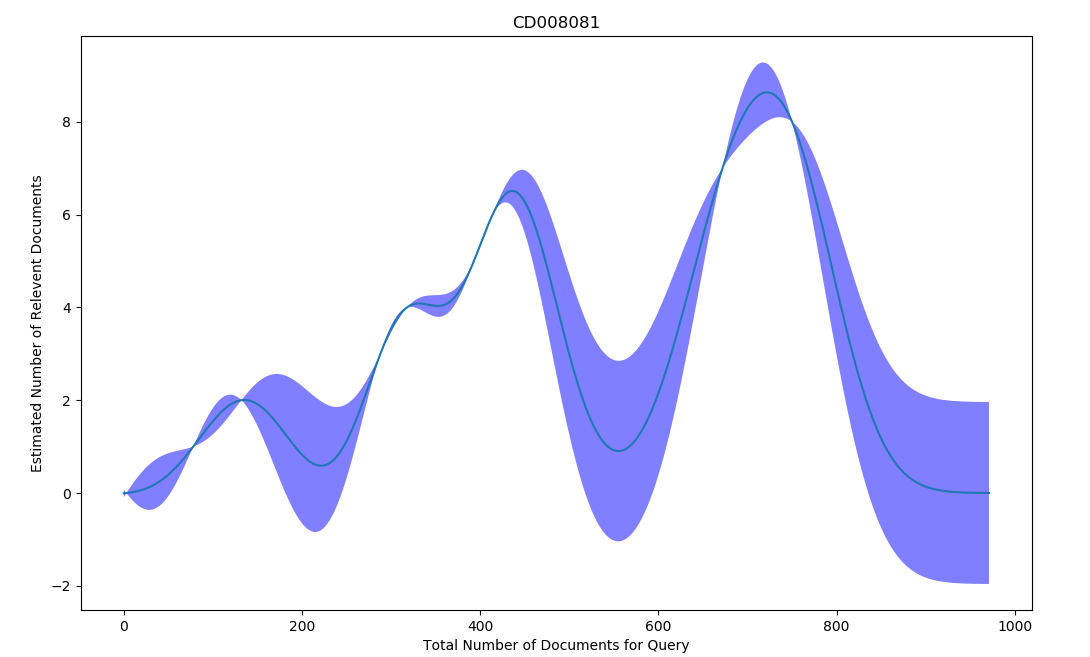
\includegraphics[width=12cm]{figures/GP_fit.png}
\caption{Visualisation of using a confidence interval for predicting a stopping point using a gp.}
\end{figure}


\subsection{Conclusion on Curve fitting and GP} \label{conclusCurveAndGp}

We implemented two methods for predicting stopping points in ranked medical studies. Our first approach used a general curve to estimate the point in which 70\% recall is likely to have been hit. Our second method used a Gaussian Process in the same way. We used a sampling method to generate our curves to makes predictions about the remaining studies.


\subsection{Comparing Methods} \label{compMethods}

\begin{table}[H]

\centering
\begin{tabular}{|c|c|c|c|c|} 
 \hline
 Method & Target & recall & reliability & effort  \\ 
 Knee Method & - & 0.888 & 0.866 & 0.640 \\
 Target Method & 10 & 0.952 & 0.960 & 0.652 \\
 Sheffield-run2-curve & - & 0.75 & 0.640 & 0.510 \\
 Sheffield-run2-cutoff(85.5\%) & - & 0.934 & 1.000 & 0.553 \\
 \hline
\end{tabular}
\caption{Comparing target method, knee, cut-off and curve fitting along with confidence interval. Using Sheffield-run-2}

\end{table}

We can evaluate how well this method does against an existing set of relevance rankings. We will use the Sheffield run data from the CLEF 2017 task \cite{Kanoulas12017}. As the target method allows us to specify our level of reliability, we needed a target $T$ of 10 to hit 95\% reliability. We can see that the reliability of our method does not come close to the Target method. Our curve, however has a much lower effort. The cut-off method described in \ref{perCutOffMethod} beats both the curve-fitting and the target methods.

Overall we believe that the Knee and Target methods are too sensitive to the ranking algorithm being used. On our Sheffield-run2 rankings we can see the performance for both these methods is significantly lower than that reported in previous work \cite{Cormack2016}



\section{Poisson Process for stopping points} \label{window_samp}

A Poisson Process can be used to model points in time in which events occur. In this situation we wish to observe the rate in which a relevant document occurs in a collection of documents.

We can observe the relevant document distribution for each topic by plotting relevant document occurrences across the whole rankings.


\begin{figure}[H]
\center
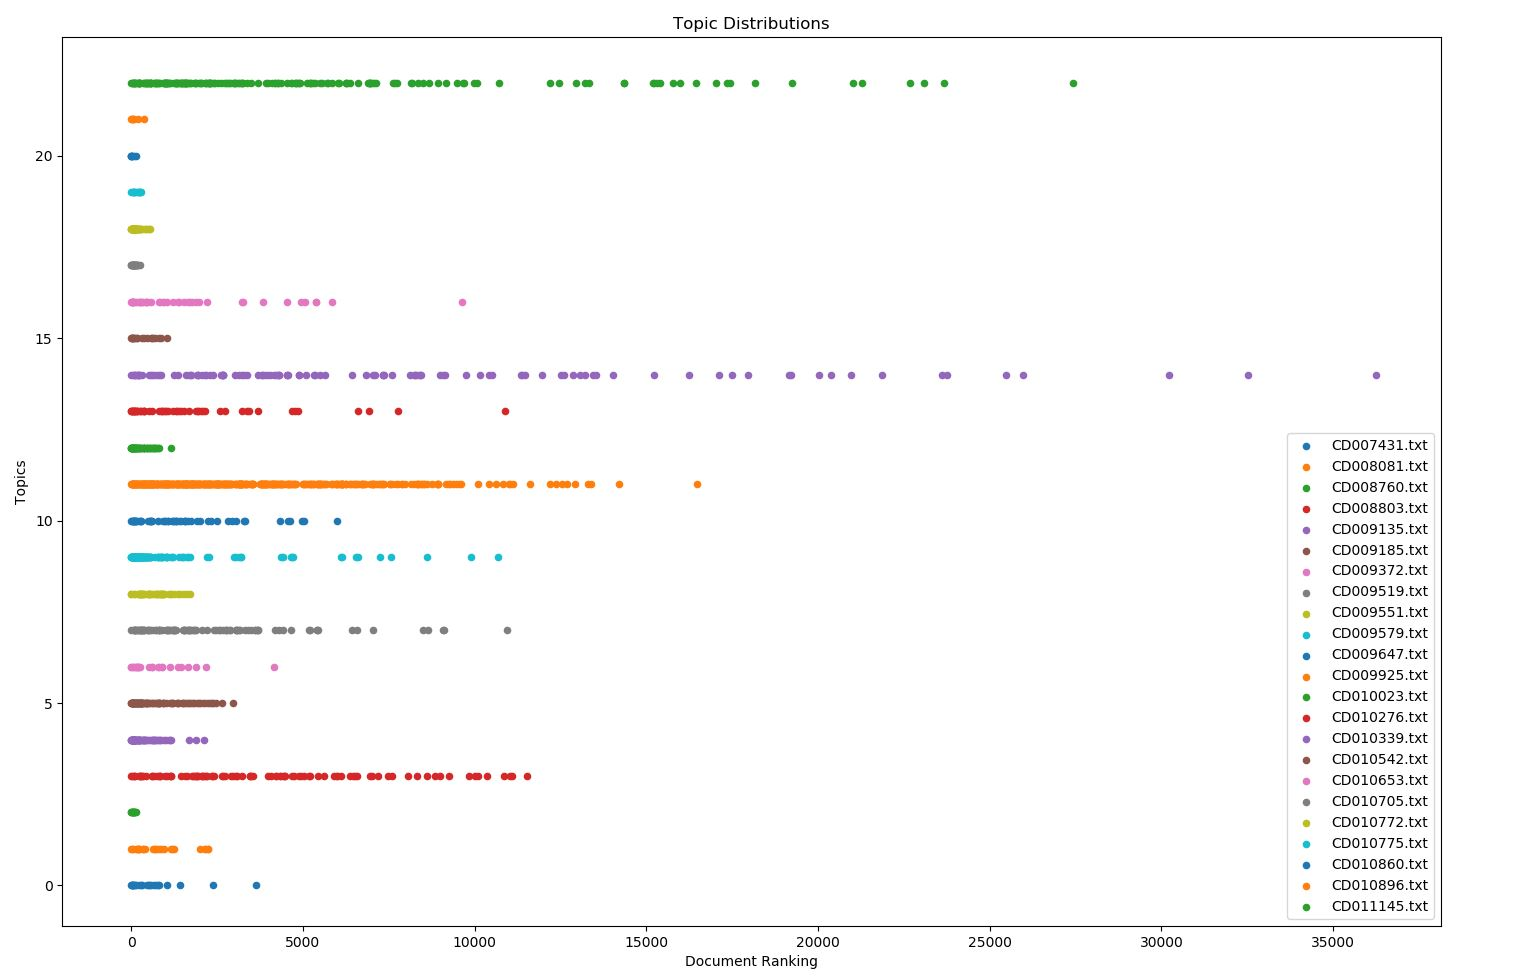
\includegraphics[width=15cm]{figures/distrib.jpg}
\caption{Relevant document distribution over Sheffield dataset}
\end{figure}

The quality of the initial rankings will determine how many relevant documents occur towards the start of the distribution. Naturally the number of relevant documents decrease as we proceed down the rankings.

The Poisson distribution is a way for us to model the occurrences of relevant documents in a fixed time-frame, in our situation, the number of documents returned by the query. To estimate the overall rate of which relevant documents occur, we can observe how many relevant documents occur within a threshold.


\begin{equation}
	  \lambda = \frac{r_i}{|D|}
\end{equation}

Where $r_i$ is the number of relevant documents in a sample set and $|D|$ is the number of documents in the sample set.

Supposing we sample 10\% of the 1000 documents, of which 7 relevant documents occur:

\begin{equation}
	  \lambda = \frac{7}{100} = 0.07
\end{equation}

We can use the rate parameter to estimate the probability of there being atleast one relevant documents, after observing $n$ documents:

\begin{equation}
	  P = 1 - e ^ {-Rn}
\end{equation}


\begin{figure}[H]
\center
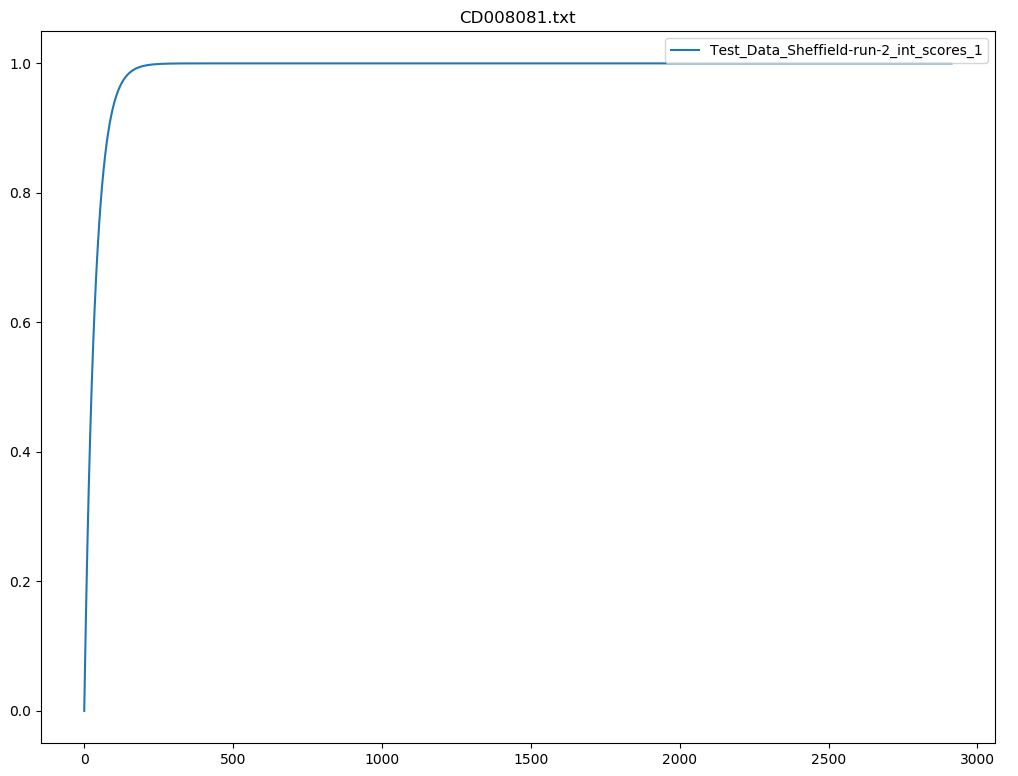
\includegraphics[width=10cm]{figures/probOneDoc.jpg}
\caption{Probability of seeing atleast one relevant document by sampling 10\% of documents for topic CD008081}
\end{figure}

The plot shows as we look at more documents, we are increasingly likely to have seen one relevant document. While this is useful to know, we can not use this as a method for predicting a suitable stopping point.

A Homogeneous Poisson Process can be used to model the occurrences of relevant document and then used to predict the probability of there bring $r$ relevant documents after $n$ documents have been observed. 

\begin{equation}
	  P(n = r) = \frac{(\lambda n)^r}{r!} e ^ {-\lambda n}
\end{equation}


Due to the high likelihood that $r!$ will be exceeding large, we can use a stirling approximation, maintaining a similar value as to what we would have obtained computing the factorial.

\begin{equation}
	   r \approx \sqrt{2\pi n} \left( \frac{r}{e} \right) ^r
\end{equation}

By summing over the probability mass from for values of $n$ between 1 and the size of the document collection we can estimate at what point 95\% reliability (stopping point $s$) is reached. 

\begin{equation}
	   s = \sum_{i \leq 0.95}^{|n|} \frac{(\lambda i)^r}{stirling(r!)} e ^ {-\lambda i}
\end{equation}

The limitation of using an Homogeneous Poisson Process is that the rate parameter is constant throughout distribution. This means if we looked at 10\% of the rankings the rate of relevant documents would be assumed to be constant for the remainder of the document collection.


\begin{figure}[H]
\center
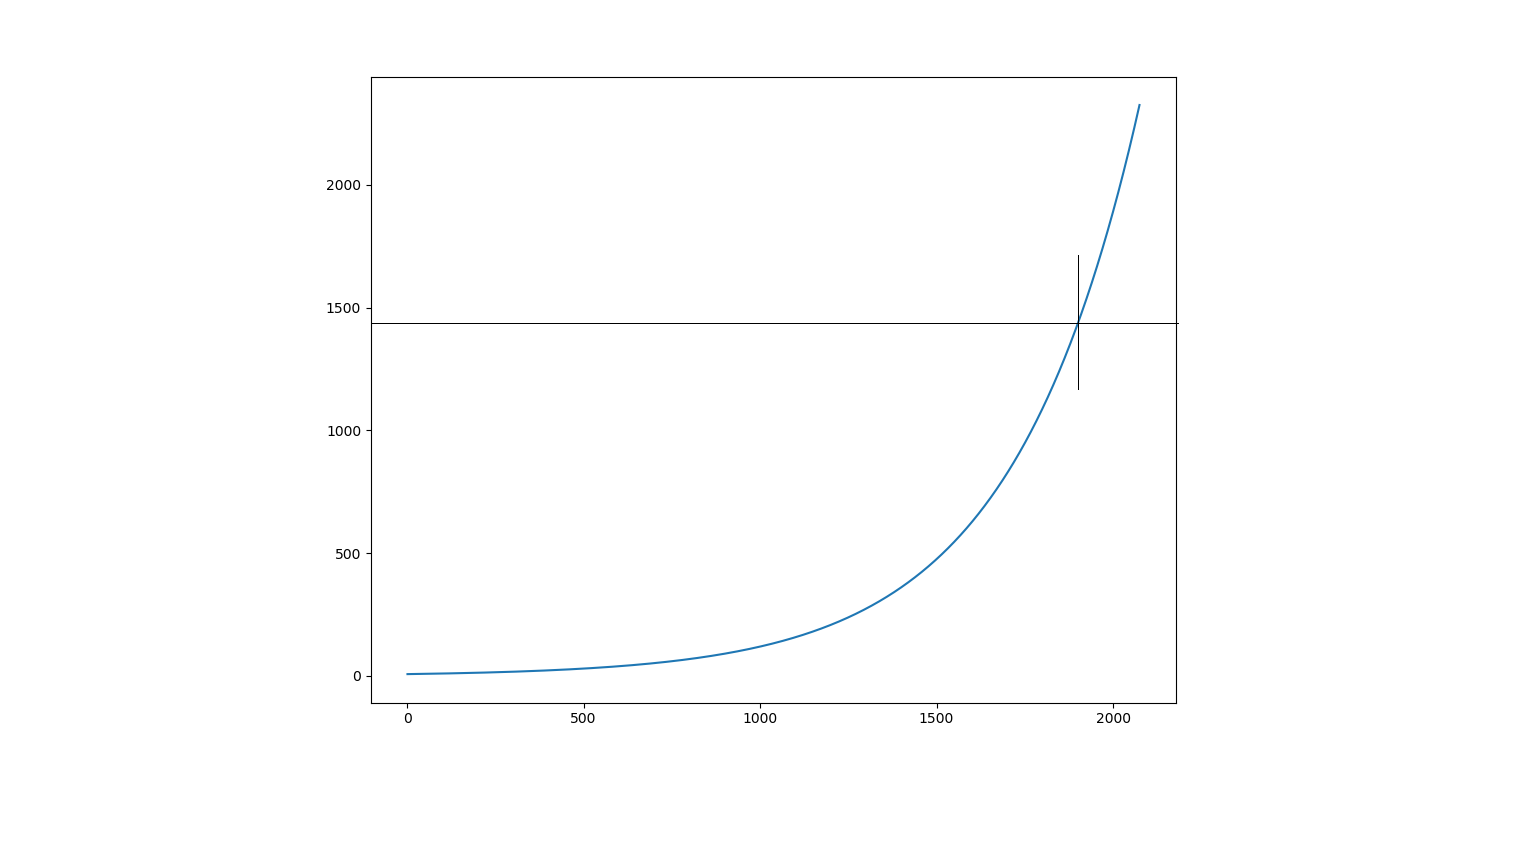
\includegraphics[width=16cm]{figures/overestimate.png}
\caption{Homogeneous Poisson Process overestimating the rate of documents, resulting a prediction curve that would expect us to look at 1500 of the 2000 documents to reach 70\% recall}
\end{figure}

\subsection{Non-Homogeneous Poisson Process}

As the rate parameter is varies throughout the distribution of documents, we can use a Non-Homogeneous Poisson Process. A Non-Homogeneous Poisson process is similar to an ordinary Poisson process, except that the average rate of arrivals is allowed to vary with time. 

\subsubsection{Window Sampling} \label{window_samp}

It is useful for us to estimate the rate in which relevant documents occur. By iterating over each document in a returned set of documents, and evaluating the relevant documents in a given window, we can estimate this rate parameter. 

\begin{table}[H]

\centering
\begin{tabular}{|c|c|c|} 
\hline
 Document Rank & Relevant & RelScore  \\ 
 1 & Y &			1/3=0.33 \\ 
 2 & Y &			3/4=0.75 \\ 
 3 & N &			4/5=0.80 \\ 
 4 & Y &			3/5 =0.60 \\ 
 5 & Y &			2/5=0.40 \\ 
 6 & N &			2/5=0.40 \\ 
 7 & N &			1/4=0.25 \\
 8 & N &			0/3=0.00 \\
  
 \hline
\end{tabular}

\caption{Using window sampling with a window size of 2 either side.}

\end{table}

By using the number of relevant documents that occur within a given window, we are able to get a declining rate distribution. 

\subsubsection{Non-Homogeneous Poisson Defination} \label{nn_pp_def}

We can use a non-homogenous poission process to estimate the number of relevant documents in a given interval by integrating the rate function $\lambda(x)$ across the interval.

We first define our intervals as $a$ and $b$ and integrate the values between them with respect to $x$

\begin{equation}
	   \int_a^b \lambda(x) d(x) = \Lambda(a, b)
\end{equation}

Therefore the probability of there being $r$ relevant documents in the interval $(a, b$)

\begin{equation}
	   P(N(a, b) = r) = \frac{[\Lambda(a,b)]^r}{r!} e^{-\Lambda(a,b)}
\end{equation}

We can make the assumption that the rate in which relevant documents appear is an exponential function.

\begin{equation}
	   \lambda(x) = ae^{kx}
\end{equation}

Therefore

\begin{equation}
	   \int_a^b \lambda(x) d(x) = \int_a^b ae^{kx} dx = \frac{a}{k}e^{kx}
\end{equation}

As we are only interested in knowing the total number of relevant documents, we can assume $a=0$ and $b=n$ where $n$ is the total number of documents.

\begin{equation}
	   \Lambda(0, n) = \int_0^n ae^{kx}dx = \frac{a}{k}e^{kx} = \frac{a}{k}(e^{kn} - 1)
\end{equation}

So

\begin{equation}
	   P(N(0,n) = r) = \frac{(\Lambda(0,n))^r}{r!}e^{-\Lambda(0,n)} = \frac{\left(\frac{a}{k}(e^{kn} -1)\right)^r}{r!} e^{-(\frac{a}{k}(e^{kn} - 1)})
\end{equation}

Therefore given values for $a$ and $k$ which we can learn from fitting an exponential curve, we can predict the probability of there being $r$ relevant documents within the entire set of $n$ documents


\section{Indexing and Querying Medline with Limited Information}

CLEF 2018 \cite{CLEFLINK} presents an appropriate sub-task for using a limited amount of information to retrieve relevant documents. Normally, reviewers are require to construct complex Boolean queries to retrieve data from Medline. The objective of CLEF 2018 Sub-Task 1: No Boolean Search \cite{CLEFLINK} is to search effectively and efficiently bypassing the construction of the Boolean query.

\subsection{Acquiring Key Information from A Systematic Review Protocol}

A systematic review protocol is created before the systematic review process is started. A systematic review protocol describes the rationale, hypothesis, and planned methods of the review. The Pubmed query is created manually with the help of the protocol. Here we are looking to generate a suitable query/relevant information from the protocol to then automatically query Pubmed.

We used RAKE \cite{rake} to extraction key-words from a protocol. The minimum word occurrence count is set to 1, as the protocols are typically small. We used a Pubmed stop list as the phrase splitting parameter. Example shown below:

\begin{tcolorbox}

Topic: CD008122 

Title: Rapid diagnostic tests for diagnosing uncomplicated P. falciparum malaria in endemic countries 

Objective: To assess the diagnostic accuracy of RDTs for detecting clinical P. falciparum malaria (symptoms suggestive of malaria plus P. falciparum parasitaemia detectable by microscopy) in persons living in malaria endemic areas who present to ambulatory healthcare facilities with symptoms of malaria, and to identify which types and brands of commercial test best detect clinical P. falciparum malaria.

\end{tcolorbox}

 
 
\begin{tcolorbox}

endemic countries objective|ambulatory healthcare facilities|rapid diagnostic tests|falciparum parasitaemia detectable|malaria endemic areas|diagnostic accuracy|falciparum malaria

\end{tcolorbox}

The | symbol represents a separation between a phrase. The protcols are pre-processed as follows: Reference removal, lowercase, words less than $N$ length removed, pubmed stoplist. We decided to not perform any stemming/additional manipulation at this stage, due to uncertainty of query format.

The key-word-query receives some final pre-processing prior to being loaded into our information retrieval (IR) system. We used a Lancaster stemmer to reduce words down to a base form. The result is as follows:

\begin{tcolorbox}

endem country object amb healthc facil rapid diagnost test falcipar parasitaem detect malar endem area diagnost acc falcipar malar

\end{tcolorbox}

\subsection{Indexing Pubmed}

Pubmed was downloaded from the online resource \footnote{https://www.ncbi.nlm.nih.gov/home/download/}. We processed the xml files and retrieved the information for each study - title, id, abstract. To reduce the size, we store each record into a local database, containing only the relevant information for each study.

We used Apache Lucene \footnote{https://lucene.apache.org/} to generate an index for the Pubmed local database. The abstract and title were concatenated together. Pre-processing was done using the same format as the query: Pubmed stoplist \footnote{https://www.ncbi.nlm.nih.gov/books/NBK3827/table/pubmedhelp.T.stopwords/}, Lancaster stemmer and lower-casing. 


\subsection{Runs}

\begin{itemize}
\item \textbf{sheffield-Boolean}  
The Sheffield Boolean runs uses words that occur the most in the document and the query as a basis for ranking. Documents that contain more query terms will feature higher in the overall rankings. We used the Apache Lucene Boolean similarity class for our implementation.\footnote{https://lucene.apache.org/core/7\_0\_1/core/org/apache/lucene/search/similarities/BooleanSimilarity.html}

\item \textbf{sheffield-tfidf} The Sheffield tfidf run uses a cosine simularity measure to compare the simularity between the query and the pubmed article. Documents and queries are represented as tfidf vectors. We used the Apache Lucene tfidf similarity class for our implementation.\footnote{https://lucene.apache.org/core/7\_0\_1/core/org/apache/lucene/search/similarities/TFIDFSimilarity.html}

\item \textbf{sheffield-bm25} This run uses the bm25 similarity measure \cite{Robertson96okapiat}. We used the Apache Lucene bm25 similarity class for our implementation.\footnote{https://lucene.apache.org/core/7\_0\_1/core/org/apache/lucene/search/similarities/BM25Similarity.html}

\end{itemize}

\subsection{Results}

Results were generated using the eval script from the CLEF 2017/2018 task \cite{Kanoulas12017}. We calculated the top $N$ results over the CLEF 2017 training set. We include a random baseline  to provide a comparison between results.


\begin{table}[H]
\scalebox{0.8}{
\centering
\begin{tabular}{|c|c|c|c|c|c|c|c|} 
 \hline
 Run & recall &  ap & lastrel & wss100 & wss95 & normarea & $N$ \\ 
 Random-baseline & 0.005 &0.002 & 126.7 &0.00 &0.00 & 0.024 & - \\
 Train-Data-Sheffield-bm25-Run1-objective-only & 0.538 &0.034 & 3039.051 &0.101 &0.108 & 0.431 & 5000 \\
 Train-Data-Sheffield-tfidf-Run1-objective-only & 0.354&0.007& 2633.718&0.021&0.023& 0.247& 5000 \\
 Train-Data-Sheffield-boolean-Run1-objective-only & 0.313 &0.034& 3039.051&0.101 &0.108 & 0.431 & 5000 \\
 Train-Data-Sheffield-bm25-Run1-objective-only & 0.680&0.034& 12310.231&0.169&0.172& 0.592& 25000 \\
 Train-Data-Sheffield-tfidf-Run1-objective-only & 0.601&0.007& 14883.744&0.13&0.136& 0.455& 25000 \\
 Train-Data-Sheffield-boolean-Run1-objective-only & 0.471&0.007& 12974.205&0.03&0.029& 0.381& 25000 \\
 
 \hline
\end{tabular}
}
\caption{Results for IR Pubmed system. Comparison for both 5000 and 25000 thresholds}
\end{table}


As we increase the number of documents we return, the recall naturally increases. When we return 25000 documents for each topic, we are able to obtain a total recall rate of over 58\%. However, the precision (ap, average precision) is very low, suggesting a significant amount of the documents are not useful. BM25 was found to be the best ranking method, followed by tfidf and boolean.

Improvements could certainly be made to this system:

\begin{itemize}
  \item MeSH headings would be useful in expanding the range of the query to capture synonymous terms. 
  \item Tokenization could be optimized to capture phrases of different sizes.
  \item Introducing a cost or stopping point to remove the amount of non-relevant documents. We can see for the 25000 documents set of results the last relevant document was around the 20000 point, meaning we could drop the last 5000 from our result set.
\end{itemize}


\subsection{Pubmed automatic query Conclusion}


We built an IR system using Apache Lucerne and compared three separate ranking methods. We found bm25 ranking gave the best results overall.

We found we were able to achieve fair results with a little optimization techniques to the index and query data.

We compared the performance of our system across different return thresholds, naturally finding as we increase the returned number of documents we get a higher recall. This comes at the expense of reduced precision.

We suggested further improvement to our system, such as including a phrase model for more robust features for both index and query.



